\documentclass[10pt]{article}
\usepackage[margin=.7in]{geometry}
\usepackage{graphicx,booktabs,hyperref,amsmath,amssymb}
\hypersetup{colorlinks=true,urlcolor=blue}
\setlength{\parindent}{0pt}
\setlength{\parskip}{6pt}
\title{Quadratic twists: native replay and checked implications}
\author{Reproducible correctness study}
\date{21 October 2026}
\begin{document}
\maketitle
\vspace{-1em}
\textbf{Outcome.} The complete finite workload now executes in C++17. All
434 deterministic output fields agree with the frozen historical results,
including newly collected IC matrices and their attempt counts. The historical
Python archive is unchanged. Eighteen Lean statements pass the
repository proof gate, with zero trusted native proofs. Universal geometric
bridges remain partial; no general hardness or speedup conclusion is drawn.

\begin{center}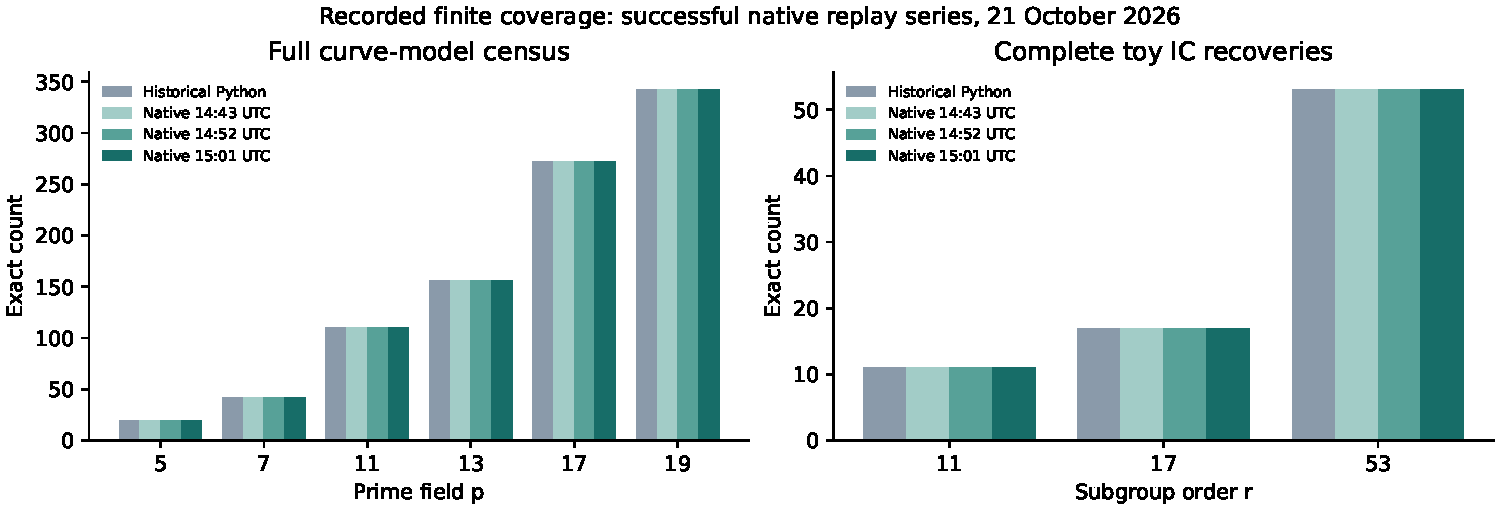
\includegraphics[width=\linewidth]{coverage.pdf}\end{center}
\small Recorded counters from the successful 14:43, 14:52 and 15:01 UTC native runs.
The earlier port attempt failed parity comparison and has no accepted result.
Exact census counts;
no statistical error bar or extrapolation. The host is uncontrolled Linux
x86-64, GCC 14.2.0 and OpenSSL 3.5.7. UTC boundaries are provenance, not admitted
algorithm timings.\normalsize

\begin{center}
\begin{tabular}{lr}
\toprule
Replayed workload & Recorded count \\\midrule
Nonsingular models, primes 5, 7, 11, 13, 17, 19 & 942 \\
Ordered S3 triples & 4,188,162 \\
Ordered S4 quadruples, primes 5 and 7 & 113,342 \\
Extension points & 260,064 \\
Twist group-law identities & 289,440 \\
Scalar transport checks & 94,176 \\
Common odd-prime cases & 274 \\
Complete toy IC logarithms & 81 \\
Bilinearity identities & 3,219 \\
\bottomrule
\end{tabular}
\end{center}

All four trace-zero fixtures, the subfield example and four transported
relation histograms match. The original 12 seeded associativity samples per
model outside prime 5 remain samples, not exhaustive proofs. Process timing,
source provenance and SymPy version fields are excluded from mathematical
parity. C++ integer-seeded MT19937 reproduces the original integer draws; exact
sparse polynomial expansion over $\mathbb Z$ replaces SymPy.

\newpage
\section*{Independent verification and controls}
The separate tuple-based auditor verifies 84 newly emitted IC matrices: three
headline runs and the 81 all-log runs. It independently recomputes the pairings,
field logarithms, scalars and ranks. Corrupting a new relation or removing a
log certificate is rejected. Changing the historical census counter is also
rejected. Existing source-corruption and false historical-relation controls remain.

Before registering the subfield target in a simple polynomial basis, the new
basis checker verifies 2,401 elements, 2,475 points and 2,025 group-map identities.
Here $u^2=3$, $v^2=1+u$, $w=v$, $u=w^2-1$, and
$w^4+5w^2+5=0$. The model catalog has 1,921 exact ICV1 models and 27 selected
EC1 subgroup representations. An unselected generator is left unknown.
The normalization of $c y^2=x^3+ax+b$ is explicit:
$(x,y)\mapsto(cx,c^2y)$ on the monic model with coefficients $c^2a,c^3b$.
No base-field log transfer is inferred from a shared model or $j$-invariant.

\section*{Proofs and experimentally discriminated claims}
The Lean module proves the mixed-relation implication: if an additive
endomorphism fixes $A$ and $A+B$ and negates $B$, then $2B=0$.
Coprime annihilators force $B=0$, proving the odd-order consequence.
The finite coprime-order homomorphism theorem, trace/anti-trace identities,
common odd-order divisor implication, three ring identities, affine twist-map
and monic-normalization equations, and algebraic embedding-degree-two
implication are also checked. All hypotheses are explicit in the proof map.
Four further statements use the actual elliptic point group, the q-power
Frobenius map and rational base-change homomorphism. Rational lifts are proved
fixed; a Frobenius-negated mixed contribution is proved killed by two and zero
under an odd annihilator. The twist-to-negation identification remains explicit.

\begin{center}\small
\begin{tabular}{ll}
S3 symmetry & \texttt{IDC1h07a9b2e6b0a3a9d3} \\
Vieta cancellation & \texttt{IDC1h98f781bdd4756596} \\
Twist equation & \texttt{IDC1hfb8edf881dcde851}
\end{tabular}\normalsize\end{center}
The records name the exact checked Lean source. Native certificate replay uses
32 derived points and 16 extra points and rejects false identities. Point
evaluation alone is weaker than the accompanying universal ring proofs.

The valid-point census retains a nonzero 2-torsion exception. S3/S4 conditions
are preserved under the geometric twist map, and the matched transported
relation histograms agree in four fixtures. All 81 pairing/IC logarithms are
recovered. A smooth or anomalous twist does not force the same original order
or a nonzero rational homomorphic transfer. The subfield fixture's order-three
target remains outside the smaller rational group. The restricted relation
family has rank 5 of 6 despite 272 smooth relations from 2,448 candidates;
a broader seeded family reaches full rank. These findings have their exact
finite scope, not an asymptotic interpretation.

\section*{Remaining obligations and provenance}
Twist embedding and its Frobenius negation property, full rational-eigenspace
identification, general summation-polynomial lifting, Weil-pairing
nondegeneracy and the full reduction, and universal trace-zero geometry remain
open bridges. General GHS construction and general ECDLP hardness are not
established. Invalid-curve attacks are outside scope. Conductor's shared tool
and task state remain unavailable. Rust and Lean are now installed; current
repository checks are recorded separately in \path{validation/}.

The original archive, import report, native source snapshots, failed first
port comparison and failed first proof build remain available. No benchmark
or leaderboard row or IC/rho cost graph is promoted. This new graph extends
study coverage; earlier reports stay attached to their original records.

\newpage
\section*{Proof map and reproduction}
\begin{center}\small
\begin{tabular}{lp{3.9in}}
\toprule
Run record & Observed outcome \\\midrule
\texttt{port-attempt-1} & Rejected: parity comparator incorrectly treated two JSON nulls as unequal. Log and exact source retained; no accepted receipt. \\
\texttt{run-20261021T144307Z} & 434 fields match; independent audit verifies 84 IC certificates. \\
\texttt{run-20261021T145210Z} & Same parity and audit; tower/simple-basis certificate added. \\
\texttt{run-20261021T150125Z} & Final source snapshot; same parity, audit and basis checks; final negative controls pass. \\
\bottomrule
\end{tabular}\normalsize\end{center}

The first 14 declarations are in \texttt{TwistProof}, with four further
declarations in \texttt{FrobeniusBridge}. Each statement's exact
hypotheses and the remaining geometric bridge are documented in
\path{lean/README.md}. The proof gate audits all 18 declarations.

\begin{center}\small
\begin{tabular}{lp{3.3in}}
\toprule
Lean declaration & Proved implication \\\midrule
\texttt{mixed\_relation\_two\_torsion} & Fixed $A$, negated $B$, fixed $A+B$ imply $2B=0$. \\
\texttt{coprime\_annihilators} & Two coprime annihilators force zero. \\
\texttt{mixed\_relation\_odd} & An odd annihilator removes the 2-torsion exception. \\
\texttt{finite\_hom\_coprime} & A homomorphism across coprime finite orders is zero. \\
\texttt{trace\_antitrace\_sum} & Trace plus anti-trace is $2P$. \\
\texttt{trace\_fixed} & An involution fixes its trace. \\
\texttt{antitrace\_negated} & An involution negates its anti-trace. \\
\texttt{common\_order\_divides\_q\_plus\_one} & An odd common order divisor divides $q+1$. \\
\texttt{symmetric\_s3} & The two S3 ring expressions agree. \\
\texttt{vieta\_twist\_cancellation} & The parameter cancels in the Vieta expression. \\
\texttt{twist\_equation\_identity} & The cleared equation is a multiple of $u^2-d$. \\
\texttt{twist\_affine\_map} & The x-fixing map satisfies the untwisted equation. \\
\texttt{monic\_normalization} & The stated scaling satisfies the monic equation. \\
\texttt{embedding\_degree\_two} & $q=-1$ and $2\ne0$ imply $q^2=1$, $q\ne1$. \\
\midrule
\multicolumn{2}{l}{\texttt{FrobeniusBridge}: actual elliptic-curve points} \\
\texttt{frobenius\_fixes\_rational} & Actual q-power Frobenius fixes rational base-change points. \\
\texttt{rational\_mixed\_two\_torsion} & A rational relation with Frobenius-negated $B$ gives $2B=0$. \\
\texttt{rational\_mixed\_odd} & With an odd annihilator, that $B$ is zero. \\
\texttt{rational\_relation\_has\_zero\_twist\_term} & $B=0$ and the two lifted rational points coincide. \\
\bottomrule
\end{tabular}\normalsize\end{center}

The group/ring implications and stated actual-point theorems are fully proved.
Identifying the embedded twist points with the minus eigenspace, and closing
the other geometric bridges, remain explicit obligations.

\begin{verbatim}
study=research/quadratic_twist_evidence_20261021
bash "$study/run-native.sh" /tmp/twist-native-fresh
bash "$study/test-native.sh" /tmp/twist-native-fresh /tmp/controls-fresh
tools/lean/proof-gate.sh --out /tmp/proofs "$study/lean"
\end{verbatim}
The adjacent Markdown report links all native records, controls, certificates,
proof receipts and the requirement map. Primary references remain in the
preserved historical report: Semaev (ePrint 2004/031), Gorla--Massierer
(arXiv 1405.1059), Menezes--Okamoto--Vanstone, and Gaudry--Hess--Smart.
\end{document}
